\documentclass{tufte-book}

\hypersetup{colorlinks}% uncomment this line if you prefer colored hyperlinks (e.g., for onscreen viewing)

%%
% Book metadata
\title{Mathematical Methods for Engineers}
\author[CAPT Stu Blair]{United States Naval Academy}
\publisher{Mighty Goat Press}

%%
% If they're installed, use Bergamo and Chantilly from www.fontsite.com.
% They're clones of Bembo and Gill Sans, respectively.
%\IfFileExists{bergamo.sty}{\usepackage[osf]{bergamo}}{}% Bembo
%\IfFileExists{chantill.sty}{\usepackage{chantill}}{}% Gill Sans

%\usepackage{microtype}

%%
% Just some sample text
\usepackage{lipsum}

%%
% For nicely typeset tabular material
\usepackage{tabularx}
\usepackage{booktabs}

%%
% For graphics / images
\usepackage{graphicx}
\setkeys{Gin}{width=\linewidth,totalheight=\textheight,keepaspectratio}
\graphicspath{{graphics/}}

% The fancyvrb package lets us customize the formatting of verbatim
% environments.  We use a slightly smaller font.
\usepackage{fancyvrb}
\fvset{fontsize=\normalsize}

%%
% Prints argument within hanging parentheses (i.e., parentheses that take
% up no horizontal space).  Useful in tabular environments.
\newcommand{\hangp}[1]{\makebox[0pt][r]{(}#1\makebox[0pt][l]{)}}

%%
% Prints an asterisk that takes up no horizontal space.
% Useful in tabular environments.
\newcommand{\hangstar}{\makebox[0pt][l]{*}}

%%
% Prints a trailing space in a smart way.
\usepackage{xspace}

%%%% packages added by Stu

\usepackage{comment}

% fancy enumeration tricks
\usepackage{enumitem}

% have appendices
\usepackage{appendix}

% has sfrac command
\usepackage{xfrac}

% mathtools for over/under brace/bracket among other nifty tools
\usepackage{mathtools}

% try to make multirow and multicolumn entries in a table.
\usepackage{array,multirow} 

\usepackage{ntheorem}
\theoremstyle{break}
\newtheorem{theorem}{Theorem}
\newtheorem{definition}{Definition}

\usepackage{cancel} % to get oblique strike-through

%\usepackage{minted}
\usepackage{pifont}
\usepackage{color}

\usepackage{listings}
\definecolor{mygreen}{rgb}{0,0.6,0}
\definecolor{mygray}{rgb}{0.5,0.5,0.5}
\definecolor{mymauve}{rgb}{0.58,0,0.82}
\lstset{ %
  backgroundcolor=\color{white},   % choose the background color; you must add \usepackage{color} or \usepackage{xcolor}
  basicstyle=\footnotesize,        % the size of the fonts that are used for the code
  breakatwhitespace=false,         % sets if automatic breaks should only happen at whitespace
  breaklines=true,                 % sets automatic line breaking
  captionpos=b,                    % sets the caption-position to bottom
  commentstyle=\color{mygreen},    % comment style
  deletekeywords={...},            % if you want to delete keywords from the given language
  escapeinside={\%*}{*)},          % if you want to add LaTeX within your code
  extendedchars=true,              % lets you use non-ASCII characters; for 8-bits encodings only, does not work with UTF-8
  frame=single,                    % adds a frame around the code
  inputpath=./matlab_examples/,
  keepspaces=true,                 % keeps spaces in text, useful for keeping indentation of code (possibly needs columns=flexible)
  keywordstyle=\color{blue},       % keyword style
  language=Matlab,                 % the language of the code
  morekeywords={*,...},            % if you want to add more keywords to the set
  numbers=left,                    % where to put the line-numbers; possible values are (none, left, right)
  numbersep=5pt,                   % how far the line-numbers are from the code
  numberstyle=\tiny\color{mygray}, % the style that is used for the line-numbers
  rulecolor=\color{black},         % if not set, the frame-color may be changed on line-breaks within not-black text (e.g. comments (green here))
  showspaces=false,                % show spaces everywhere adding particular underscores; it overrides 'showstringspaces'
  showstringspaces=false,          % underline spaces within strings only
  showtabs=false,                  % show tabs within strings adding particular underscores
  stepnumber=2,                    % the step between two line-numbers. If it's 1, each line will be numbered
  stringstyle=\color{mymauve},     % string literal style
  tabsize=2,                       % sets default tabsize to 2 spaces
  title=\lstname                   % show the filename of files included with \lstinputlisting; also try caption instead of title
}

% example usage for code: \begin{lstlisting}[caption=< caption text >, label=<label>]

%%% end packages added by Stu
%%
% Some shortcuts for Tufte's book titles.  The lowercase commands will
% produce the initials of the book title in italics.  The all-caps commands
% will print out the full title of the book in italics.
\newcommand{\vdqi}{\textit{VDQI}\xspace}
\newcommand{\ei}{\textit{EI}\xspace}
\newcommand{\ve}{\textit{VE}\xspace}
\newcommand{\be}{\textit{BE}\xspace}
\newcommand{\VDQI}{\textit{The Visual Display of Quantitative Information}\xspace}
\newcommand{\EI}{\textit{Envisioning Information}\xspace}
\newcommand{\VE}{\textit{Visual Explanations}\xspace}
\newcommand{\BE}{\textit{Beautiful Evidence}\xspace}

\newcommand{\TL}{Tufte-\LaTeX\xspace}

% Prints the month name (e.g., January) and the year (e.g., 2008)
\newcommand{\monthyear}{%
  \ifcase\month\or January\or February\or March\or April\or May\or June\or
  July\or August\or September\or October\or November\or
  December\fi\space\number\year
}


% Prints an epigraph and speaker in sans serif, all-caps type.
\newcommand{\openepigraph}[2]{%
  %\sffamily\fontsize{14}{16}\selectfont
  \begin{fullwidth}
  \sffamily\large
  \begin{doublespace}
  \noindent\allcaps{#1}\\% epigraph
  \noindent\allcaps{#2}% author
  \end{doublespace}
  \end{fullwidth}
}

% Inserts a blank page
\newcommand{\blankpage}{\newpage\hbox{}\thispagestyle{empty}\newpage}

\usepackage{units}

% Typesets the font size, leading, and measure in the form of 10/12x26 pc.
\newcommand{\measure}[3]{#1/#2$\times$\unit[#3]{pc}}

% Macros for typesetting the documentation
\newcommand{\hlred}[1]{\textcolor{Maroon}{#1}}% prints in red
\newcommand{\hangleft}[1]{\makebox[0pt][r]{#1}}
\newcommand{\hairsp}{\hspace{1pt}}% hair space
\newcommand{\hquad}{\hskip0.5em\relax}% half quad space
\newcommand{\TODO}{\textcolor{red}{\bf TODO!}\xspace}
\newcommand{\na}{\quad--}% used in tables for N/A cells
\providecommand{\XeLaTeX}{X\lower.5ex\hbox{\kern-0.15em\reflectbox{E}}\kern-0.1em\LaTeX}
\newcommand{\tXeLaTeX}{\XeLaTeX\index{XeLaTeX@\protect\XeLaTeX}}
% \index{\texttt{\textbackslash xyz}@\hangleft{\texttt{\textbackslash}}\texttt{xyz}}
\newcommand{\tuftebs}{\symbol{'134}}% a backslash in tt type in OT1/T1
\newcommand{\doccmdnoindex}[2][]{\texttt{\tuftebs#2}}% command name -- adds backslash automatically (and doesn't add cmd to the index)
\newcommand{\doccmddef}[2][]{%
  \hlred{\texttt{\tuftebs#2}}\label{cmd:#2}%
  \ifthenelse{\isempty{#1}}%
    {% add the command to the index
      \index{#2 command@\protect\hangleft{\texttt{\tuftebs}}\texttt{#2}}% command name
    }%
    {% add the command and package to the index
      \index{#2 command@\protect\hangleft{\texttt{\tuftebs}}\texttt{#2} (\texttt{#1} package)}% command name
      \index{#1 package@\texttt{#1} package}\index{packages!#1@\texttt{#1}}% package name
    }%
}% command name -- adds backslash automaticallygit@github.com:stu314159/Nuclear_Plant_Engineering.git
\newcommand{\doccmd}[2][]{%
  \texttt{\tuftebs#2}%
  \ifthenelse{\isempty{#1}}%
    {% add the command to the index
      \index{#2 command@\protect\hangleft{\texttt{\tuftebs}}\texttt{#2}}% command name
    }%
    {% add the command and package to the index
      \index{#2 command@\protect\hangleft{\texttt{\tuftebs}}\texttt{#2} (\texttt{#1} package)}% command name
      \index{#1 package@\texttt{#1} package}\index{packages!#1@\texttt{#1}}% package name
    }%
}% command name -- adds backslash automatically
\newcommand{\docopt}[1]{\ensuremath{\langle}\textrm{\textit{#1}}\ensuremath{\rangle}}% optional command argument
\newcommand{\docarg}[1]{\textrm{\textit{#1}}}% (required) command argument
\newenvironment{docspec}{\begin{quotation}\ttfamily\parskip0pt\parindent0pt\ignorespaces}{\end{quotation}}% command specification environment
\newcommand{\docenv}[1]{\texttt{#1}\index{#1 environment@\texttt{#1} environment}\index{environments!#1@\texttt{#1}}}% environment name
\newcommand{\docenvdef}[1]{\hlred{\texttt{#1}}\label{env:#1}\index{#1 environment@\texttt{#1} environment}\index{environments!#1@\texttt{#1}}}% environment name
\newcommand{\docpkg}[1]{\texttt{#1}\index{#1 package@\texttt{#1} package}\index{packages!#1@\texttt{#1}}}% package name
\newcommand{\doccls}[1]{\texttt{#1}}% document class name
\newcommand{\docclsopt}[1]{\texttt{#1}\index{#1 class option@\texttt{#1} class option}\index{class options!#1@\texttt{#1}}}% document class option name
\newcommand{\docclsoptdef}[1]{\hlred{\texttt{#1}}\label{clsopt:#1}\index{#1 class option@\texttt{#1} class option}\index{class options!#1@\texttt{#1}}}% document class option name defined
\newcommand{\docmsg}[2]{\bigskip\begin{fullwidth}\noindent\ttfamily#1\end{fullwidth}\medskip\par\noindent#2}
\newcommand{\docfilehook}[2]{\texttt{#1}\index{file hooks!#2}\index{#1@\texttt{#1}}}
\newcommand{\doccounter}[1]{\texttt{#1}\index{#1 counter@\texttt{#1} counter}}

% Generates the index
\usepackage{makeidx}
\makeindex

\begin{document}

\begin{fullwidth}
\thispagestyle{empty}
\begin{figure}
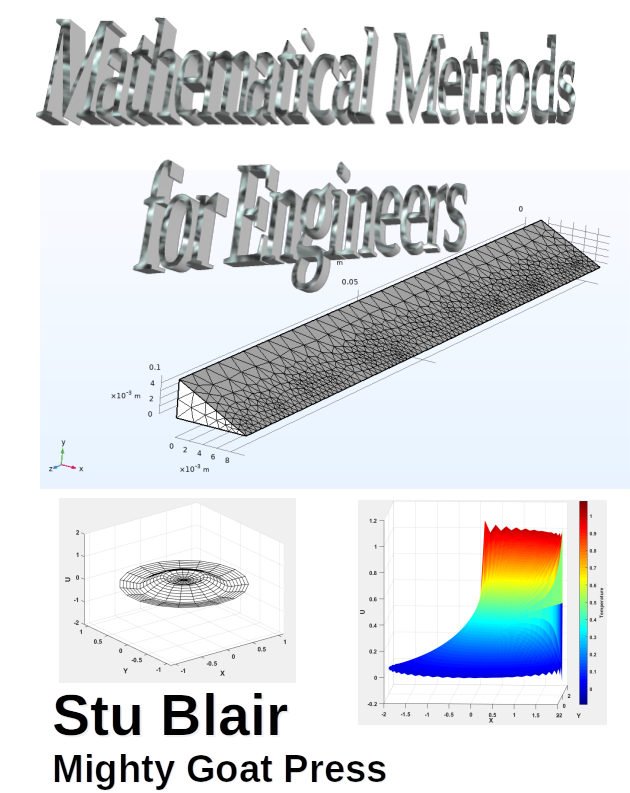
\includegraphics[width=1.5\textwidth]{cover1.png}
\end{figure}
\end{fullwidth}

% Front matter
\frontmatter

% r.1 blank page
%\blankpage


% v.2 epigraphs
\newpage\thispagestyle{empty}
\vfill
\openepigraph{%
When in doubt, multiply both sides by an orthogonal function and integrate.
}{P.L. Chebyshev}

\vfill
\openepigraph{%
The purpose of computing is insight, not pictures
}{L.N. Trefethen}


\vfill
\openepigraph{%
Never do a calculation until you already know the answer.
}{J.A. Wheeler}


% r.3 full title page
\maketitle


% v.4 copyright page
\newpage
\begin{fullwidth}
~\vfill
\thispagestyle{empty}
\setlength{\parindent}{0pt}
\setlength{\parskip}{\baselineskip}
Copyright \copyright\ \the\year\ \thanklessauthor
\par\smallcaps{Published by \thanklesspublisher}

%\par\smallcaps{tufte-latex.github.io/tufte-latex/}
%
%\par Licensed under the Apache License, Version 2.0 (the ``License''); you may not
%use this file except in compliance with the License. You may obtain a copy
%of the License at \url{http://www.apache.org/licenses/LICENSE-2.0}. Unless
%required by applicable law or agreed to in writing, software distributed
%under the License is distributed on an \smallcaps{``AS IS'' BASIS, WITHOUT
%WARRANTIES OR CONDITIONS OF ANY KIND}, either express or implied. See the
%License for the specific language governing permissions and limitations
%under the License.\index{license}

\par\textit{First printing, \monthyear}
\end{fullwidth}

% r.5 contents
\tableofcontents

\listoffigures

\listoftables

% r.7 dedication
%\cleardoublepage
%~\vfill
%\begin{doublespace}
%\noindent\fontsize{18}{22}\selectfont\itshape
%\nohyphenation
%Dedicated to the midshipmen of the United States Naval Academy; the future of our armed services and of %our country.
%\end{doublespace}
%\vfill
%\vfill


% r.9 introduction
\cleardoublepage
\chapter*{Preface}

The purpose of this text is to provide a concise reference for engineering students who would like to strengthen their conceptual understanding and practical proficiency in analytical and numerical methods in engineering.  The material is based on a sequence of two courses taught at the United States Naval Academy.  

\subsection*{Analytical Methods}

The first course focused on analytical methods for linear ordinary and partial differential equations.  All students came into the course having taken a three-semester sequence of calculus along with a course in ordinary differential equations.  The analytical methods portion quickly reviews methods for constant coefficient linear equations and proceeds to methods for non-constant coefficients including Cauchy-Euler equations, power series methods, and method of Frobenieus.  After a review of Fourier Series methods and an introduction to Fourier-Legendre and Fourier-Bessel expansions we thoroughly explore solutions to second-order, linear, partial differential equations.  Since many students are also studying nuclear engineering, there is a heavy focus on addressing boundary value problems in cylindrical and spherical coordinate systems that are applicable to other topics of interest such as reactor physics.  There is also heavy emphasis on heat transfer applications that students will see later on in their undergraduate curriculum.

The materials presented are based heavily on Professor Dennis Zill's excellent book.\cite[-3cm]{zill2020advanced} We lightly select from chapters 1-3 for review; chapter 5 for series solution methods; and chapters 12-14 for Fourier Series and solutions to linear boundary value problems.  Material from that text is used throughout this book.  

What distinguishes this course from Prof Zill's work is the incorporation of computational tools in the solution process.  These ``semi-analytical methods'' are presented here in MATLAB\cite[-3.75cm]{matlab} owing to the students preparation with that tool.  Other open-source tools like Octave\cite[-3.5cm]{octave} and Python,\cite[-1cm]{10.5555/1593511} of course, could be used. 

\subsection*{Numerical Methods}

%%
% Start the main matter (normal chapters)
\mainmatter

\part{Introduction and Review}

\chapter{Lecture 1 - Course Introduction and Numeric Preliminaries}
\label{ch:lec1n}
\section{Objectives}
The objectives of this lecture are:
\begin{itemize}
\item Introduce the course objectives.
\item Describe how numbers are represented on computers.
\item Outline sources of errors in numerical methods relative to analytical methods.
\end{itemize}
\setcounter{lstannotation}{0}

\section{Course Introduction}

This course is intended to be an introduction and overview of numerical methods.\marginnote[-0.5cm]{\textbf{Question:} What are numerical methods? 

\vspace{0.25cm}

\noindent \textbf{Answer:} Numerical methods (or numerical analysis) is the study of \emph{algorithms} for the problems of \emph{continuous} mathematics.}  The target audience comprises undergraduate students of engineering who have already taken a full sequence of calculus and differential equations courses.  Some students may also have taken the analytical methods course described earlier in this book. All students are expected to have some proficiency in the MATLAB programming environment.  

\subsection{Objectives}
\newthought{The objectives} for this course are as follows:

\begin{enumerate}
\item Students will understand the fundamentals of numerical methods with an emphasis on the most essential algorithms and methods.

\item Students will have enhanced their scientific computing skills and further developed their proficiency in using the MATLAB environment to implement algorithms and have learned to critically evaluate their results.

\item Students will understand the fundamentals of the finite element method (FEM) and have attained an introductory-level proficiency in using the COMSOL software package to carry out a multi-physics analysis of a relevant physical model.

\item Students will have developed the ability to formulate a problem of interest, apply numerical methods and computational tools to analyze the problem, and communicate pertinent results to others.
\end{enumerate}


\subsection{Course Topics}
The specific topics we will cover include:

\begin{enumerate}
\item Methods for solving non-linear equations
\begin{enumerate}
\item Bisection method
\item Newton's method
\item Secant method

\end{enumerate}
\item Methods for solving linear equations
\begin{enumerate}
\item Gauss elimination and related methods like LU- and Cholesky factorization
\item Iterative solution methods for sparse linear systems of equations\sidenote{We will also discuss some preconditioners.}
\end{enumerate}
\item Curve fitting
\begin{enumerate}
\item Least squares algorithms
\item Curve fitting with Lagrange polynomials
\end{enumerate}
\item Numeric differentiation
\begin{enumerate}
\item Finite difference methods
\item Lagrange polynomials
\end{enumerate}
\item Numeric integration
\begin{enumerate}
\item A variety of Newton-Cotes methods
\item Gauss Quadrature
\end{enumerate}

\item Initial- and Boundary-value problems \sidenote{This section will prominently include MATLAB built-in methods; particularly for boundary value problems.}
\begin{enumerate}
\item Runge-Kutta methods for initial value problems\sidenote{We will not extensively cover either explicit or implicit multi-step methods, giving preference to the wide variety of very effective RK methods.}
\item Shooting method for boundary value problems
\item Finite element method\sidenote{There will be a simple MATLAB demonstration with application to one-dimensional boundary value problems.  The majority of FEM coverage will be related to the use of COMSOL.}
\end{enumerate}

\end{enumerate}  

\vspace{4.0cm}

\section{Representation of Numbers on a Computer}

Every engineer who uses computational tools in their work should have a basic understanding of how numbers are represented on a computer.  The essential take-aways from this section are:
\begin{enumerate}
\item Since the computer is a finite machine, only a finite set of numbers can be exactly represented on the computer.  All other numbers are approximated.
\item Computers store integers and non-integers differently and the limits to what numbers can be represented or how exactly they are represented are also different.
\item The fact that numbers, in general, are represented inexactly on the computer has an impact on how algorithms are developed.
\end{enumerate}

\subsection{Integers}
Integers are represented exactly on a computer, but only a finite subset of all integers can be represented.  There are a number of integer types that are supported by common computer architectures and language compilers.\marginnote[-4.5cm]{Some of the integer data types specified by the C++ language standard include:
\begin{enumerate}
\item signed char (8 bits)
\item short int (16 bits)
\item int (at least 16 bits -- usually 32 bits)
\item long int (at least 32 bits)
\item long long int (at least 64 bits)
\end{enumerate}
Each of these categories includes a signed and unsigned variant.  Even within these categories there is fuzziness---e.g. \emph{``at least 16 bits''}---that allows for variations between different compiler implementations and computer hardware (e.g. Intel vs. AMD CPU).
}\marginnote{\textbf{Note:} The word \emph{bit} is taken to be synonymous with the words \emph{binary digit}.} For the purposes of this class we will focus on two types: \emph{unsigned integers} and \emph{signed integers}.  To further focus the discussion we will only consider 32-bit representations of signed and unsigned integers.

\newthought{Perhaps the easiest} integer representation to understand is the 32-bit unsigned integer.\sidenote{You can create a 32-bit unsigned integer in MATLAB by typing:

\vspace{0.1cm}

\noindent \lstinline[style=myMatlab]{x = uint32(1994)}

\vspace{0.1cm}

Variables with other data types can be constructed using similar syntax; see the MATLAB documentation for details.
} In this format 32 binary digits corresponding to $2^0$ to $2^{31}$ are stored in memory.  Numbers in binary work the same way our normal decimal number work: just base 2 instead of base 10.  For example, the 32-bit unsigned integer representation of the number 23 is shown in Figure \ref{fig:lec1n-binary-23}.


\begin{figure}[h!]
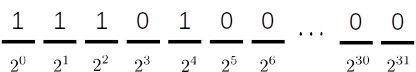
\includegraphics[width=0.75\columnwidth]{binary_23.png}
\caption{The number 23 in unsigned integer format.}
\label{fig:lec1n-binary-23}
\end{figure}


%\vspace{0.25cm}
%\noindent (image of 24 in binary)
%\vspace{0.25cm}

With 32-bit unsigned integers the computer can exactly represent all integers between 0 and $2^{32}-1$. Negative integers and integers greater than $2^{31}$ are not represented at all.%\sidenote{\textbf{Question:} What do you get from the following MATLAB code?
%\begin{lstlisting}[style=myMatlab]
%a = uint32(2^32-1);
%b = uint32(1);
%c = a + b;
%fprintf('c = %d \n',c);
%\end{lstlisting}

%\lstinline[style=myMatlab]{ a = uint32(2^32 - 1)  b = unit32(1) }

%\vspace{0.1cm}

%\noindent\textbf{Answer:} The variable c will still be equal to $2^{31}-1$.  MATLAB will round numbers outside of the range of representation for 32-bit unsigned ints to the nearest endpoint which, in this case, is $2^{31}-1$.
%}

\newthought{There are fewer} applications for which \emph{signed integers} will be used for this course, but they are, naturally, important.  Perhaps the most obvious way that a computer might represent signed integers would be to just use the same format as unsigned integers except to reserve one bit for the sign.  This is not, however, the way it is normally done.  For one thing, this approach results in there being two different bit-patterns for zero.  This might seem like a trivial inconvenience but it is not the sort of thing that passes without notice in computer engineering circles. Another, perhaps more significant, issue with this approach is that special logic would be needed when adding or subtracting a mixture of positive and negative integers. (i.e. you would not be able to use the same circuitry on the microprocessor for adding positive and negative numbers together as you would for adding two positive numbers.)
  
The format that is normally used today for representing signed integers is called \emph{two's complement}.  If you want to write a positive number in two's complement format, you do the same thing as you would normally do for an unsigned integer.\sidenote[][-1.5cm]{Except, as it turns out, the largest positive 32-bit signed integer will only half as large as the corresponding largest signed integer.} If you need to write a negative number, you start by expressing the positive number, then you \emph{take the complement of each binary digit} and, when you are done with that, you \emph{add one.} A demonstration of this number representation, shortened to 5-bits to make it more compact, is shown in Figure \ref{fig:twos-complement-demo}.  


\begin{marginfigure}
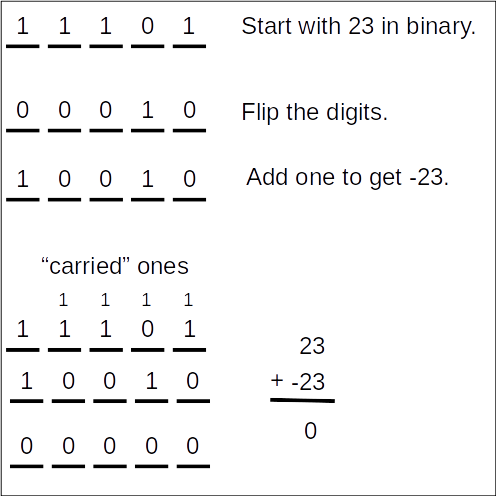
\includegraphics{twos-complement-demo.png}
\caption{Demonstration of twos-complement: adding 23 and -23 in 5-bit representation.}
\label{fig:twos-complement-demo}
\end{marginfigure}

%\vspace{0.25cm}
%\noindent (image showing example two's complement)
%\vspace{0.25cm}

This representation has the advantages that: a) there is only a single representation for zero; and b) the same hardware is used for both addition and subtraction (i.e. to subtract you simply add a negative number.)

\subsection{Floating Point Numbers}
In general, binary floating point numbers are given in the form shown in Equation \ref{eq:bfpn-format}:
\begin{equation}
1.\underbrace{\text{fff}\dots\text{f}}_{\text{mantissa}} \times 2^{\underbrace{\text{eee}\dots\text{e}}_{\text{exponent}}}
\label{eq:bfpn-format}
\end{equation}
where a number of digits available are divided between the fraction, or \emph{mantissa}, and \emph{exponent}.  In any finite machine, there will be a limit to the number of total digits available.  Thus an engineering decision needs to be made to determine how many digits will be allocated to the mantissa and how many for the exponent.  If you have more digits in the mantissa, you will be able to represent numbers that are closer together---the \emph{precision} of your representation will increase.  If you allocate more digits to the exponent, you will be able to represent numbers that are larger (for large positive exponents) or smaller (large negative exponents)---the \emph{range} of your representation will be wider.  The implications of these decisions should be clear: if you devote fewer bits to the mantissa, there will be more rounding errors in your calculations as real numbers are mapped, in some way, to the best floating point representation; if you devote fewer bits to the exponent, really large numbers and really small numbers will not be represented at all.  In earlier days of computing, different computer vendors made different decisions as to how floating point numbers would be represented.\cite{moler_fp1}  This caused problems when scientists tried to run the same code on different computers and got different results.  In 1985, the IEEE-754 standard was approved and, since then, has been adopted by essentially all computer manufacturers.  As a result, the menagerie of floating point formats and implementations have been tamed. Scientists and engineers could run their codes on different machines and expect to get the same results.

\begin{figure}
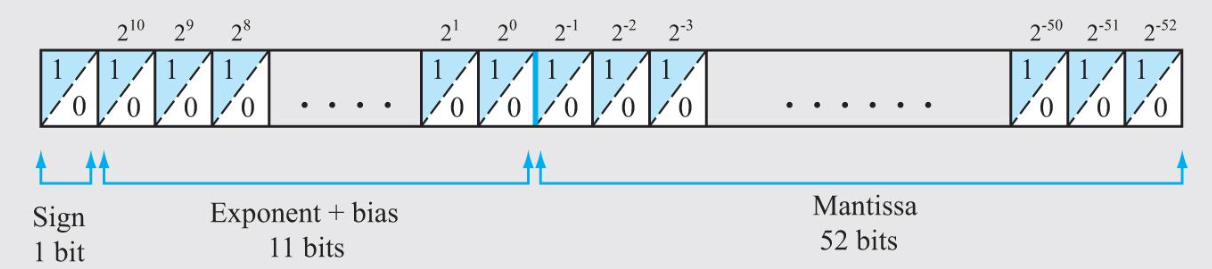
\includegraphics[width=0.94\columnwidth]{double-precision-format.png}
\caption{IEEE-754 double precision number format.}
\label{fig:double-precision-format}
\end{figure}

The IEEE-754 standard provides specification of several floating point number formats.  For this class, we will be concerned primarily with the \emph{double precision} floating point format which is illustrated in Figure \ref{fig:double-precision-format}.  This format uses a single sign bit (1 for negative, 0 for positive), 11 bits for the exponent which is encoded as an unsigned integer with bias,\sidenote{For double precision numbers, the bias is 1023.} and 52 bits for the mantissa.\sidenote{\textbf{Note:} The number 1 shown in Equation \ref{eq:bfpn-format} is not stored but is implicitly included in all \emph{normalized} floating point numbers.  This is done so that all numbers will have a \emph{unique} floating point representation. }  In the double precision format, the smallest positive number that can be represented is $2^{-1022}$ which is approximately equal to $2.2 \times 10^{-308}$.\marginnote{MATLAB includes built-in functions to report the smallest and largest representable floating point numbers.  The functions \lstinline[style=myMatlab]{realmin(precision)} and \lstinline[style=myMatlab]{realmax(precision)} will return the  smallest or largest positive floating point number for ``single'' or ``double'' precision floating point precision.} The smallest interval between numbers that can be represented is called \emph{machine epsilon}.\marginnote{In MATLAB, machine epsilon is provided with the function: \lstinline[style=myMatlab]{eps(precision)} for ``single'' and ``double'' precision.}  The size of this limit is driven by the number of bits in the mantissa.  For IEEE-754 double precision floating point numbers this is approximately $2.22 \times 10^{-16}$.\sidenote{Sometimes computational scientists refer to this as ``16 digits of precision.''}

\newthought{The procedure to} encode real numbers in the double precision floating point format will be illustrated with an example.

\vspace{0.5cm}

\noindent\textbf{Example:} Write the number -10.5 using the IEEE-754 double precision format.

\vspace{0.25cm}

\noindent\textbf{Step \#1:} Determine the mantissa and the exponent.  To do this, we normalize the number by dividing by $2^e$ where $e$ is the largest power of 2 that is \emph{less} than the magnitude of the number you are encoding.  

\vspace{0.1cm} 

\noindent In this case, $e=3$ since 10.5 is greater than $2^3$ but less than $2^4$.  

\begin{align*}
\frac{-10.5}{2^3} & = -1.3125 \\
\Rightarrow -10.5 &= -1.3125 \times 2^3
\end{align*}

\noindent Therefore the mantissa will need to encode 0.3215, and the exponent will need to encode 3 plus the bias of 1023, or 1026.

\vspace{0.25cm}

\noindent\textbf{Step \#2:} Set the sign bit. As the number is negative, the sign bit is: 1.

\vspace{0.25cm}


\noindent\textbf{Step \#3:} Calculate the 11 exponent bits.  

\begin{align*}
1026 &= 1024 + 2 \\
&= 1 \times 2^{10} + 1 \times 2^{1}
\end{align*}


\begin{figure}
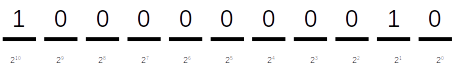
\includegraphics[width=0.75\columnwidth]{lec1n-ex1-exponent.png}
\caption{Exponent: 3+1023 = 1026 in 11-bit binary.}
\label{fig:lec1n-ex1-exponent}
\end{figure}   
  

\vspace{0.25cm}

\noindent\textbf{Step \#4:} Calculate the 52 mantissa bits to represent 0.3125.  The result is shown in Figure \ref{fig:lec1n-ex1-mantissa}.

\begin{figure}
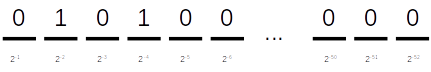
\includegraphics[width=0.75\columnwidth]{lec1n-ex1-mantissa.png}
\caption{Mantissa: 0.25 + 0.0625 = 0.3125.}
\label{fig:lec1n-ex1-mantissa}
\end{figure}

\noindent Where the calculations might be done as shown below:
\begin{align*}
0.3125 - 0 \times 2^{-1} &= 0.3125 \\
0.3125 - 1 \times 2^{-2} &= 0.0625 \\
0.0625 - 0 \times 2^{-3} &= 0.0625 \\
0.0625 - 1 \times 2^{-4} &= 0
\end{align*}
and all other entries are, of course, zero.


\section{Sources of Error} \index{error, truncation} \index{error, round-off} \index{error, modeling}

When using numerical methods there are several sources of error that you, as an engineer, should be aware of.  We have just discussed the details of double precision numbers so \emph{round-off error} is at the top of our mind.  Real numbers are not represented exactly on a computer but instead as floating point numbers.  The floating point number \emph{closest} to the real number gets used in its place. Error due to this round-off accumulates with mathematical operations.  Quantitative analysis of the accumulation of round-off-error is a tedious (albeit important) business that we will avoid in this class.  Nonetheless, engineers need to be aware that it is happening and, in a few instances, we will take steps to mitigate this build-up of error.

The second source of error that we will mention here is something that should be familiar to students who have taken the course in analytical methods: \emph{truncation error}.  In the analytical methods course we suffered from truncation error every time we shortened our infinite series solution to a finite number of terms.  We reduced this error by increasing the number of terms we retained, but there was no way to make it go away completely.  In this course we will see further instances of truncation error in most every algorithm we implement.  Derivatives and integrals that could, in principle, be done exactly, will be done approximately as we truncate the Taylor series expansion or limit the order of polynomials used to represent the exact derivative or integral.  We can reduce the magnitude of these errors, but we cannot make them go away entirely.

The third source of error mentioned here is \emph{modeling error}.  Modeling errors are reflected in the differences between observed physical phenomena and the corresponding mathematical model of the phenomena.  There are a couple of reasons for these differences and these include:
\begin{enumerate}
\item Linearization of non-linear processes.  Instances where you may already have done this, in your heat transfer or fluid dynamics class, include:
\begin{enumerate}
\item Assumption of constant thermal conductivity for heat conduction problems.  This assumption linearizes the heat equation and, for simple geometry, renders the problem amenable to analytical methods.  This assumption is retained for many numerical methods when solving the heat equation on more complex geometry.  The modeling error resulting from linearization remains.

\item Assumption of constant drag coefficient for external flow calculations.  Once again, this assumption simplifies the calculations at the cost of model fidelity.
\end{enumerate}

\item De-coupling of physical processes.  Nature does not specialize its behavior by academic subjects.  Consequently the air flowing over the control surfaces of a fighter jet is both a fluid dynamics and structural dynamics problem when the wing responds to forces imposed by the air.  Water flowing through a pressurized water reactor core is heated by forced convection and radiation that you might calculate in heat transfer class, but the resulting change in water properties also affect the neutron economy and power production rate that you might calculate in reactor physics which, in turn, will have further effect on the heat transfer problem.  We de-couple these processes so the analysis is more manageable but as a result the solution we arrive at is in error.  

\end{enumerate}  
Scientists and engineers need to be aware of all of these sources of errors and take steps to mitigate them where possible.




\chapter{Lecture 2 - Separable and Linear 1st order Equations}
\label{ch:lec2}
\section{Objectives}
The objectives of this lecture are:
\begin{itemize}
\item Define and describe the solution procedure for \emph{separable} first order equations
\item Define and demonstrate the solution procedure for \emph{linear} first order equations
\end{itemize}

\section{Separable Equations}
A first order differential equation of the form shown below
\begin{equation}
\frac{du}{dx} = g(u)h(x)
\label{eq:separable}
\end{equation}
is said to be \emph{separable} or have \emph{separable variables.}\marginnote[-1.5cm]{\textbf{Note:} there is \textbf{no} requirement that the 1st order equation be \emph{linear}.  This is one of the few techniques that we will study in this course that can be applied to nonlinear equations.} 

\newthought{The solution method} for separable equations is, in princple simple.  For the separable differential equation given in Equation \ref{eq:separable} we would separate and integrate:

\begin{align*}
\frac{du}{dx} &= g(u)h(x) \\
\frac{du}{g(u)} &= h(x) dx \\
\int \frac{1}{g(u)} \ du &= \int h(x) \ dx 
\end{align*}
\marginnote[-3.5cm]{\textbf{Note:} there are at least two complications here.
\begin{enumerate}
\item The solution you thus derive may be either implicit or explicit.  An implicit solution is, as a practical matter, fairly inconvenient to deal with; and
\item It may not be possible to actually carry out the integrals analytically. 
\end{enumerate}
Nonetheless, we shall carry on and give it a try anyway.  
}
Generally speaking, one of your first checks for a first order equation should be: is it separable?  If so, you should separate the variables and solve.  The examples below are intended to illustrate the method.  Note that in the final example, the integral cannot be done analytically.
\begin{example}[h!]
Solve the following separable, first order differential equations
.
\textbf{Example 1:} 
\begin{align*}
\frac{du}{dx} &= \frac{u}{1 + x} \\
\frac{du}{u} &= \frac{dx}{1+x} \\
\int \frac{d}{u} &= \int \frac{dx}{1+x} \\
\ln{|u|} + c_1 &= \ln{|1+x|} + c_2 \\
|u| &= e^{\left[\ln{|1+x|} + c_3\right]}\\
    u(x)&= c|1+x|
\end{align*}

\end{example}

\begin{example}[h!]
\textbf{Example 2:}
\begin{align*}
\frac{du}{dx} &= -\frac{x}{u} \\
\int u \ du &= -\int x \ dx \\
\frac{u^2}{2} &= -\frac{x^2}{2}+c \\
u(x) &= \sqrt{c - x^2}
\end{align*}
\end{example}

\begin{example}[h!]
\textbf{Example 3:}
Solve the first order initial value problem shown below:
\begin{equation}
\frac{du}{dx} = e^{-x^2}, \ \ u(2) = 6, \ \ 2 \le x < \infty
\end{equation}
\begin{align*}
du &= e^{-x^2}\ dx \\
\int_2^{x} \frac{du}{dt} \ dt &= \int_{2}^{x} e^{-t^2} \ dt \\
u(x) - u(2) &= \int_{2}^{x} e^{-t^2} \ dt \\
u(x) &= 6 + \int_{2}^{x} e^{-t^2} \ dt
\end{align*}
where we have used the dummy variable $t$ in the integrals; the last integral will need to be evaluated numerically.

\end{example}

\section{Linear Equations}
A first-order differential equation of the form:
\begin{equation}
a_1(x)\frac{du}{dx} + a_0(x)u = g(x)
\label{eq:lin_first_order}
\end{equation}
is said to be a first order \emph{linear equation} in the dependent variable $u$.\marginnote[-2.0cm]{\textbf{Note:} it is sometimes customary to write the differential equation in \emph{operator form} where the differential operator, $\mathcal{L}=a_1(x) \frac{d}{dx} + a_0(x)$, is applied to the function $u(x)$ to get $g(x)$; $\mathcal{L}u(x) = g(x)$ }
When $g(x) = 0$, the first-order linear equation is said to be \emph{homogeneous}; otherwise it is \emph{nonhomogeneous}.\marginnote{Notice that $g(x)$ is the only term in Equation \ref{eq:lin_first_order} that does \underline{\textbf{not}} include $u$ or any of its derivatives.}

\newthought{When solving} equations of this type it is useful to express it in the \textbf{standard form}:
\begin{equation}
\frac{du}{dx}+P(x)u = f(x)
\label{eq:first-order-linear-standard-form}
\end{equation}  
The method for solving this equation makes use of the \underline{\emph{linearity}} property\marginnote{When we say an operator is \textbf{linear}, what we mean is that the following relationships must hold:
\begin{enumerate}
\item $\mathcal{L}(\alpha u) = \alpha \mathcal{L}(u)$
\item $\mathcal{L}(u + v) = \mathcal{L}(u) + \mathcal{L}(v)$
\end{enumerate}
for functions $u$,$v$ and scalar constant $\alpha$.  Think of this as a \emph{definition} of linearity.} and express the solution in the following way: $u(x) = u_c(x) + u_p(x)$; plugging this into Equation \ref{eq:first-order-linear-standard-form} gives us:

\begin{multline}
\frac{d}{dx}[u_c + u_p] + P(x)[u_c + u_p] = \\
\left[\frac{du_c}{dx}+P(x)u_c \right] + \left[\frac{du_p}{dx}+P(x)u_p \right] = f(x) 
\label{eq:lin-first-order1}
\end{multline}
where $u_c(x)$ is the solution to the \emph{associated homogeneous problem}\marginnote{The linear operator here is: $\mathcal{L}=\frac{d}{dx} + P(x)$.  Equation \ref{eq:fol_complementary} says $\mathcal{L}u_c = 0$; Equation \ref{eq:fol_particular} says $\mathcal{L}u_p = f(x)$; Equation \ref{eq:lin-first-order1} says that $\mathcal{L}(u_c+u_p) = 0+f(x) = f(x)$.}
\marginnote[0.25cm]{What might trouble you now is: if we have $u_p$, is this not a solution to Equation \ref{eq:first-order-linear-standard-form}?  Why do we need $u_c$?  The next thing that should trouble you is that if $u_p$ is a solution, by the linearity property of $\mathcal{L}$, so is $u_p$ plus \emph{any} constant multiple of $u_c$.  The solution is not \emph{unique}}
\marginnote[0.25cm]{This will all be resolved when we recall that $u_c$ will have an arbitrary constant through which we will be able to say that $u = u_c + u_p$ is a function describing \emph{all} possible solutions of Equation \ref{eq:first-order-linear-standard-form} and the arbitrary constant in $u_c$ will be set so as to uniquely satisfy a given initial/boundary condition.}
\begin{equation}
\frac{du_c}{dx}+P(x)u_c = 0
\label{eq:fol_complementary}
\end{equation}
and $u_p(x)$ is the solution to:
\begin{equation}
\frac{du_p}{dx}+P(x)u_p = f(x)
\label{eq:fol_particular}
\end{equation}
We can see that Equation \ref{eq:fol_complementary} is separable:
\begin{align*}
\frac{du_c}{dx}+P(x)u_c &= 0 \\
\frac{du_c}{u_c} &= -P(x) \ dx \\
\ln{u_c} + C &= -\int_{P(x) \ dx} \\
u_c(x) &= e^{-\int P(x) \ dx + C_1} \\
u_c(x) &= e^{-\int P(x) \ dx}e^{C_1}
u_c(x) &=Ce^{-\int P(x) \ dx}
\end{align*}
where $C = e^{C_1}$.\marginnote{\textbf{Note:} At some point in time, I will desist in making such piddling distinctions between constants.  $C_1$ is an arbitrary constant, $e^{C_1}$ is still an arbitrary constant; there is no real difference between $C_1$ and $C$ and, in this author's humble opinion, they do not rate different symbols.}

\newthought{We need to find} a solution $u_p(x)$ to Equation \ref{eq:fol_particular}.  The technique we will use is called \emph{variation of parameters}.  It consists of looking for a solution in the form $y_p(x) = v(x)u_1(x)$, where $u_1(x) = e^{-\int P(x) \ dx}$ which is $u_c(x)$ with the arbitrary constant set to 1 and $v(x)$ might be thought of as some kind of weighting or \emph{variational} function.

\newthought{We will insert} this proposed form of $y_p(x)$ into Equation \ref{eq:fol_particular}:
\begin{equation*}
\frac{d(vu_1)}{dx} + P(x)(v(x)u_1(x))=f(x)
\end{equation*}
We apply the product rule to the first term and re-arrange terms:
\begin{align*}
u_1(x)\frac{dv}{dx}+ v(x)\frac{du_1}{dx} + P(x)(v(x)u_1(x)) &= f(x) \\
v(x)\underbrace{\left[\frac{du_1}{dx}+P(x)u_1(x) \right]}_{\textbf{= 0}}+u_1(x)\frac{dv}{dx} &= f(x) \\
u_1(x)\frac{dv}{dx} &= f(x)
\end{align*}
In the last line we can observe that the equation is \emph{separable} and thus solve:
\begin{align*}
v(x) &= \int \frac{f(x)}{u_1(x)} \ dx \\
     &= \int e^{\int P(x) \ dx}f(x) \ dx
\end{align*}
Now that we know what $v(x)$ must be, we can combine this with $u_1(x)$ to get $u_p(x)$:
\begin{equation}
u_p(x) = e^{-\int P(x) \ dx}\left[\int e^{\int P(x) \ dx}f(x) \ dx \right]
\label{eq:fol-particular-sol}
\end{equation}
Equation \ref{eq:fol-particular-sol} is messy and perhaps a bit scary but given definitions of $P(x)$ and $f(x)$ we might hope we can solve it anyway.  We now have expressions for both $u_c$ and $u_p$; they can be combined into the solution for the first-order linear equation:
\begin{equation}
u(x) = Ce^{-\int P(x) \ dx} + e^{-\int P(x) \ dx} \left[e^{\int P(x) \ dx} f(x) \ dx \right]
\label{eq:fol-solution}
\end{equation}

\section{Method of Solution}
Once we have identified a problem to be first-order and linear, we will solve the problem using the following steps:
\begin{enumerate}
\item Write the equation in standard form (Equation \ref{eq:first-order-linear-standard-form})
\item Determine the integrating factor $\mu = e^{-\int P(x) \ dx}$.
\item Solve for the general solution $u(x)$ using Equation \ref{eq:fol-solution}.
\item Apply initial/boundary condition if given.
\end{enumerate}

\vspace{1cm}
\underline{\textbf{Example:}}
Solve the problem:
$$\frac{du}{dx}+u=x, \ \ u(0) = 4$$

\textbf{Solution:}

\textbf{Step 1:}
The equation is already in standard form, so this step is easy.

\vspace{0.25cm}
\textbf{Step 2:} Find the integrating factor $\mu$.

$$mu = e^{-\int P(x) \ dx} = e^{-\int 1 \ dx} = e^{-x}$$

\vspace{0.25cm}
\textbf{Step 3:} Solve for the general solution $u(x)$ using Equation \ref{eq:fol-solution}
\marginnote[1.25cm]{$\leftarrow$ For the integral $\int e^x x \ dx$ we need to use integration by parts.}
\begin{align*}
u(x) &= Ce^{-x}+e^{-x}\int e^{x}x \ dx \\
&= Ce^{-x} + e^{-x}\left[xe^{x}-e^{x} \right] \\
&= Ce^{-x} + x - 1
\end{align*}

\vspace{0.25cm}
\textbf{Step 4:} Apply initial/boundary conditions if given

\begin{align*}
u(0) &= Ce^{0} + 0 -1 \\
 &=C-1 = 4 \\
 \Rightarrow C &= 5 \\
 u(x) &= 5e^x+x-1
\end{align*}




\chapter{Assignment \#1}
\label{ch:ass1n}
\begin{fullwidth}

\begin{enumerate}
\item Write the number 38.8125 as a 64-bit double-precision string using the IEEE-754 standard. 



\vspace{2.0cm}

\item In single precision (IEEE-754 standard), 8 bits are used for storing the exponent (the bias is 127), and 23 bits are used for storing the mantissa.  What (approximately) are the smallest and largest positive numbers that can be stored in single precision?

\vspace{2.0cm}

\item The value of $\pi$ can be calculated with the series:
\begin{equation*}
\pi = 4 \sum\limits_{n=1}^{\infty} (-1)^{n-1}\frac{1}{2n-1} = 4 \left(1 - \frac{1}{3} + \frac{1}{5} - \frac{1}{7} + \frac{1}{9} - \frac{1}{11} + \cdots \right)
\end{equation*}
Write a MATLAB script that calculates the value of $\pi$ by using $n$ terms of the series and calculate the corresponding true relative error.  Calculate $\pi$ and the true relative error for $n=10$, 20, and 40. \textbf{Note:} Implement the partial series summation as a \emph{local function} named \lstinline[style=myMatlab]{piApprox} that takes one argument---the number of terms ($n$)---and returns the estimated value of $\pi$ and the true relative error.  Use MATLAB's built-in constant \lstinline[style=myMatlab]{pi} for the ``true'' value of $\pi$.

\vspace{2.0cm}

\item Using a hand calculator, determine the root of $f(x)=x-2e^{-x}$ with the bisection method.  Start with $a=0$ and $b=1$, and carry out the first three iterations to determine an estimated root and bracket within which the root lies.

\vspace{2.0cm}

\item Write a MATLAB user-defined function that solves for a root of a nonlinear equation $f(x)=0$ using the bisection method.  Implement the function as a \emph{local function} that takes three arguments: \lstinline[style=myMatlab]{fun}, \lstinline[style=myMatlab]{a}, and \lstinline[style=myMatlab]{b}, where \lstinline[style=myMatlab]{fun} is a handle to the nonlinear function for which a root is to be found and \lstinline[style=myMatlab]{a} and \lstinline[style=myMatlab]{b} bracket the root.  The bisection iterations should stop when $f(x_{\text{NS}})\le 0.0000001$ where $x_{\text{NS}}$ is the midpoint of the current bracket.  The function should also check if points \lstinline[style=myMatlab]{a} and \lstinline[style=myMatlab]{b} do indeed bracket a root; if not, the function should return an error message.  Use your function to find the root of $f(x) = x-2e^{-x}$.  


\vspace{2.0cm}
\index{van der Waals equation}
\item The van der Waals equation gives a relationship between the pressure $P$ (in atm.), volume $V$ (in liters), and temperature $T$ (in K) for a real gas:
\begin{equation}
P = \frac{nRT}{V-nb}-\frac{n^2 a}{V^2}
\label{eq:ass1n-van-der-waals}
\end{equation}
where $n$ is the number of moles, $R=0.08206$ (L-atm)/(mole-K) is the gas constant, and $a$ (in L\textsuperscript{2}-atm/mole\textsuperscript{2}) and $b$ (in L/mole) are material constants.  Consider 1.5 moles of nitrogen ($a$=1.39 L\textsuperscript{2}-atm/mole\textsuperscript{2}) at 25$^{\circ}$C stored in a pressure vessel.  Use the function you created for problem \#5 to determine the volume of the vessel if the pressure is 13.5 atm.


\end{enumerate}

\end{fullwidth}

\chapter{Lecture 3 - Theory of Linear Equations}
\label{ch:lec3}
\section{Objectives}
The objectives of this lecture are:
\begin{itemize}
\item Introduce several theoretical concepts relevant to initial value problems and boundary value problems.
\item Demonstrate use of the Wronskian to determine linear independence of solutions.
\item Present some important theorems and definitions relevant to the theory of linear ordinary differential equations.
\end{itemize}

\section{Initial Value Problems}

For a linear differential equation, an n\textsuperscript{th}-order initial value problem (IVP) is given by the following governing equation and initial conditions:
\begin{equation}
\text{Governing Equation: }a_n(x)\frac{d^n u}{dx^n}+a_{n-1}\frac{d^{n-1}u}{dx^{n-1}}+\cdots+a_1(x)\frac{du}{dx}+a_0(x)u=g(x)
\label{eq:ivp-ge}
\end{equation}
\begin{equation}
\text{Initial Conditions: }u(x_0)=u_0, \ u^{\prime}(x_0)=u_1,\dots,u^{(n-1)}(x_0)=u_{n-1}
\label{eq:ivp-ics}
\end{equation}
\marginnote[-1.5cm]{\textbf{Note:} for an initial value problem, all of the initial conditions are provided at the same value of $x$; in accordance to custom we call this $x_0$.  The name \emph{initial} condition gives the implication that these conditions are at some ``end'' of the interval (beginning, left side, whatever) and in most all examples and exercises this is indeed the case.  It is \underline{not}, however, a requirement.}
\noindent \newthought{We seek a} function defined on some interval containing $x_0$ that satisfies the differential equation with $n$ conditions applied.\marginnote{Generally for an n\textsuperscript{th}-order IVP you will need $n$ conditions.} The theorem below, which we will use by \emph{citing} rather than \emph{proving}, gives us assurance that, subject some fairly reasonable assumptions, such a solution will exist.  

\begin{theorem}[Existence and Uniqueness for IVPs]
If $a_n(x),a_{n-1}(x),\dots,a_1(x),a_0(x)$ and $g(x)$ are continuous on an interval $\mathcal{I}$, and if $a_n(x) \ne 0$ for every $x \in \mathcal{I}$, and if $x_0$ is any point in this interval, then a solution $u(x)$ of the IVP exists on the interval and it is unique.
\label{thm:IVP-exist-and-unique}
\end{theorem}
\newthought{For this class} we will adopt a mostly operational definition of continuity: if you can draw the function throughout the specified interval without picking up your pencil or without diverging to infinity, then the function is continuous.  

Consider, as an example, the following initial value problem:
\begin{equation}
u^{\prime \prime}-4u = 12x, \ \ u(0)=4, \ u^{\prime}(0)=1
\end{equation}
This IVP satisfies the conditions of Theorem \ref{thm:IVP-exist-and-unique} since all of the coefficients and $g(x)$ are continuous and $a_1$ is constant and nonzero; hence a unique solution exists on any interval and that solution is unique.\marginnote[-1.5cm]{Take a moment to verify that $u(x)=3e^{2x}+e^{-2x}-3x$ satisfies both the governing equation and initial conditions and thus is \emph{the} unique solution to this IVP.}

Here is an IVP that does \emph{not} satisfy the criteria of Theorem \ref{thm:IVP-exist-and-unique}:
\begin{equation}
x^2u^{\prime \prime} - 2xu^{\prime}+2u=6, \ \ u(0)=3, \ u^{\prime}(0)=1
\label{eq:lec3-ex2}
\end{equation}
\noindent In this case, the coefficients and $g(x)$ are all continuous but $a_2(x)$ is equal to zero at $x=0$.  This might not be a problem---i.e. if $x=0$ is not in the interval of interest for the IVP then we are okay---but since $x_0=0$, $x=0$ \emph{must} be in the domain for the theorem to apply.  So we have no assurances that a solution exists or, if a solution does exist, it may not be unique.\marginnote[-1.5cm]{You should take a moment to verify that $u(x)=cx^2+x+3$ is a solution for the IVP given in Equation \ref{eq:lec3-ex2} for \emph{any} choice of parameter $c$.}

\section{Boundary Value Problems}
For this section let us, without undue loss of generality, consider a 2\textsuperscript{nd}-order boundary value problem (BVP):\marginnote{Almost all of the applications we will consider for this class will involve 2\textsuperscript{nd}-order operators.  The way we derive important boundary-value problems from underlying physical laws like conservation of mass and conservation of energy lead to them being 2\textsuperscript{nd}-order.  You should think about this while you are sitting in your fluid dynamics class and equations are being derived for conservation of mass and momentum for viscous incompressible fluid flow or when you are sitting in heat transfer class and the heat equation is being derived from conservation of energy principles.  Probably the most obvious counterexample is beam theory which involves a 4\textsuperscript{th}-order operator.}
\begin{equation}
\text{Governing Equation: }a_2(x)\frac{d^2u}{dx^2}+a_1(x)\frac{du}{dx}+a_0(x)u=g(x) 
\end{equation}
\begin{equation}
\text{Boundary Conditions: } y(a)=y_0, \ \ y(b)=y_1, \ \ a \ne b
\end{equation}

\newthought{Depending on the} boundary conditions, BVPs may have no solutions, one unique solution, or infinitely many solutions.

\vspace{1.0cm}
\noindent \underline{\textbf{Example:}} The equation $u^{\prime \prime}+16u = 0$ has the general solution $u(t) = c_1 \cos{(4t)}+c_2 \sin{(4t)}$.  Consider the three different sets of boundary conditions provided below.
\begin{enumerate}[label=\alph*)]
\item $x(0)=0, \ \ x(\pi/2)=0$
Application of the first boundary condition gives us $c_1(1)+c_2(0)=0 \Rightarrow c_1 = 0$.  The second boundary condition is $c_2\sin{(2 \pi)} = 0,$ which is true for \emph{any} value of $c_2$.  Therefore there problem has infinitely many solutions.
\item $x(0)=0, \ \ x(\pi/8)=0$
The first boundary condition again gives us $c_1=0$; the second condition $c_2\sin{(4 \frac{\pi}{8})}=0$ is only satisfied if $c_2=0$.  Thus $c_1 = c_2 = 0$; only the trivial solution, $u=0$, satisfies both the differential equation and boundary conditions.  This is not a very interesting solution but at least it \emph{is a solution} so we will take this as an example of a BVP having a unique solution.\marginnote{For applications, we will generally be only interested in \emph{non-trivial} solutions; that is, solutions that are not identically equal to zero.}
\item $x(0)=0, \ \ x(\pi/2)=1$
In this case, again $c_1=0$ from the first boundary condition.  This leaves the second boundary condition: $c_2 \sin{\left(4 \frac{\pi}{2}\right)} = c_2(0) = 1$ which cannot be satisfied for any value of $c_2$.  In this case \emph{no} solution exists.

\end{enumerate}

\section{Superposition and Linear Dependence}
In this section some important theorems regarding IVPs and BVPs will be presented.  No attempt will be made to prove these theorems; we will simply take these theorems as facts that are relevant for this course that you should try to understand as best you can.

\begin{theorem}[Superposition Principle for Homogeneous Equations]
Let $u_1,u_2,\dots,u_k$ be solutions of a homogeneous n\textsuperscript{th}-order linear differential equation.  Then any linear combination of those solutions 
$$u = c_1u_1+c_2u_2+\cdots+c_ku_k$$where $c_1,c_2,\dots,c_k$ are arbitrary constants, is also a solution.
\end{theorem}
\marginnote[-3.0cm]{\textbf{Note:} It is essential that \emph{both} the governing equation and given conditions (boundary or initial) for the linear differential equation are homogeneous.  As a reminder, this means that \emph{all} terms in the governing equation and boundary conditions must either a) involve the dependent variable or one of its derivatives; or b) be equal to zero.} 
As an example, If I denote the linear homogeneous differential equation as $\mathcal{L}$, then $\mathcal{L}(u_i) = 0$ for any $i \in [1,2,\dots,k]$.  By the linearity property of $\mathcal{L}$, for any constants $\alpha$ and $\beta$:
\begin{align*}
\mathcal{L}(\alpha u_i + \beta u_j) &=  \alpha \mathcal{L}(u_i) + \beta \mathcal{L}(u_j)\\
&= \alpha(0) + \beta(0) \\
&= 0
\end{align*}

\begin{theorem}[Linear Dependence / Independence of Functions]
A set of functions $f_1(x),f_2(x),\dots,f_k(x)$ is said to be \emph{linearly dependent} on an interval $\mathcal{I}$ if there exist constants $c_1,c_2,\dots,c_k$, \emph{not \underline{all} of which are zero}, such that
$$c_1f_1(x) + c_2f_2(x)+\cdots+c_kf_k(x) = 0$$
\noindent for every $x \in \mathcal{I}$.  If the set of functions is \emph{not} linearly dependent, it is linearly independent.
\label{th:linear-dep}
\end{theorem} 
\marginnote[-1.75cm]{What if a member of the set of functions is $f(x)=0$? 

\vspace{0.25cm}

\noindent\textbf{Answer:} The set will no longer be linearly independent.  The trivial function $f(x)=0$ is not linearly independent from \emph{anything}.}
Repeatedly throughout this course we will want to clarify whether or not two or more functions are linearly independent of each other.  I think most engineers have a general idea of what it is we \emph{mean} when we say two functions are linearly independent or dependent but Theorem \ref{th:linear-dep} specifies what these things mean \emph{mathematically}.  
\newthought{We need a test} to help us determine if the members of a set of functions are linearly independent or not. This will be especially important as we evaluate solutions to a linear homogeneous differential equation.  Even if you are the sort of savant who can, by inspection, always detect linear dependence, you might have a hard time convincing your friends that your assessment is always correct.  Luckily, there is a theorem that provides a suitable test that can serve as irrefutable evidence of the state of linear dependence/independence of functions.

\begin{theorem}[Criterion for Linearly Independent Solutions]
Let $u_1,u_2,\dots,u_n$ be solutions of a homogeneous linear n\textsuperscript{th}-order differential equation defined on an interval $\mathcal{I}$.  Then the set of solutions is linearly independent on the interval if and only if the Wronskian of the solution is non-zero for every $x \in \mathcal{I}$.  
\end{theorem}\index{Wronskian}
The Wronskian is a function that takes functions as arguments and returns a scalar numeric quantity.\sidenote{Sometimes such functions are referred to as \emph{functionals}.}
\begin{equation}
W(u_1,u_2,\dots,u_n)=
\begin{vmatrix}
u_1 & u_2 & \cdots & u_n \\
u^{\prime}_1 & u^{\prime}_2 & \cdots & u^{\prime}_n \\
\vdots & \vdots & \vdots & \vdots \\
u^{(n-1)}_1 & u^{(n-1)}_2 & \cdots & u^{(n-1)}_n
\end{vmatrix}
\label{eq:Wronskian-def}
\end{equation}
where $|\cdot|$ denotes the matrix determinant.  For large values of $n$ this is also difficult to calculate but, for the case $n=2$, engineering students should be familiar with the formula:
\begin{equation}
W(u_1,u_2) = 
\begin{vmatrix}
u_1 & u_2 \\
u^{\prime}_1 & u^{\prime}_2 \\
\end{vmatrix}
= u_1 u^{\prime}_2 - u^{\prime}_1 u_2
\end{equation}

\vspace{0.5cm}

\noindent\textbf{\underline{Example:}} show that the functions $u_1 = e^{3x}$ and $u_2=e^{-3x}$ are linearly independent solutions to the homogeneous linear equation $u^{\prime \prime}-9u=0$ for every $x \in (-\infty,\infty)$.

\noindent\textbf{\underline{Solution:}} The Wronskian is given by:\marginnote{The reader should verify that both $u_1 = e^{3x}$ and $u_2=e^{-3x}$ satisfy the given differential equation.}
\begin{align*}
W &= 
\begin{vmatrix}
e^{3x} & e^{-3x} \\
3e^{3x} & -3e^{-3x}
\end{vmatrix} \\
&= e^{3x}\left(-3e^{-3x}\right) - 3e^{3x}\left(e^{-3x}\right) \\
&= 3e^{3x-3x} - 3e^{3x-3x} \\
&= 3 - 3 \\
&= 6
\end{align*}
\noindent Since $6 \ne 0$ for all $x \in (-\infty,\infty)$ the solutions are linearly independent.

\begin{definition}[Fundamental Set of Solutions]
Any set $u_1,u_2,\dots,u_n$ of $n$ linearly independent solutions of the homogeneous linear n\textsuperscript{th}-order differential equation on an interval is said to be a fundamental set of solutions on an interval $\mathcal{I}$.  
\end{definition}
\begin{theorem}[Existence of a Fundamental Set]
There exists a fundamental set of solutions for the homogeneous linear n\textsuperscript{th}-order differential equation on an interval $\mathcal{I}$.
\end{theorem}
\marginnote[-1.0cm]{\textbf{Note:} This is different than saying that a BVP or IVP has a solution.  This theorem is only referring to the differential equation; not the boundary or initial conditions.}

\begin{definition}[General Solution---Homogeneous Equation]
Let $u_1,u_2,\dots,u_n$ be a fundamental set of solutions to the homogeneous linear n\textsuperscript{th}-order differential equation defined on an interval $\mathcal{I}$, then the general solution is:
$$u(x) = c_1u_1(x)+c_2u_2(x)+\cdots+c_nu_n(x)$$
\end{definition}

\newthought{It is important} to understand from the above that:
\begin{itemize}
\item \emph{any} possible solution to the homogeneous, linear, n\textsuperscript{th}-order differential equation can be constructed by setting the coefficients of the general solution; and
\item there is \textbf{no} solution that can be constructed from functions that are linearly independent from the general solution.
\end{itemize}

\section{General Solution for a Non-homogeneous Problem}
Recall: ``non-homogeneous'' for a linear n\textsuperscript{th}-order differential equation means that $g(x)\ne 0$.  if $u_p$ is any particular solution to the non-homogeneous, linear, n\textsuperscript{th}-order ODE on an interval $\mathcal{I}$ and $u_c = c_1u_1(x) + c_2u_2(x)+\cdots c_nu_n(x)$ is the general solution to the associated homogeneous ODE (called the \emph{complementary} solution) then the general solution to the non-homogeneous ODE is:
\begin{equation*}
u = u_c + u_p
\end{equation*}

\vspace{0.25cm}

\noindent\textbf{\underline{Example:}} By substitution it can be seen that $u_p = -\frac{11}{12}-\frac{1}{2}x$ is a particular solution to $u^{\prime \prime \prime}-6u^{\prime \prime} + 11u^{\prime} - 6u=3x$.  The general solution to the associated homogeneous problem is $u_c = c_1e^{x}+c_2e^{2x}+c_3e^{3x}$.\marginnote{You are, again, strongly encouraged to verify that $u_p$ satisfies the given equation and that $u_c$ satisfies the associated homogeneous equation.}  Consequently, the general solution to the linear non-homogeneous problem is:
\begin{align*}
u(x) &= u_c + u_p \\
&=c_1e^{x}+c_2e^{2x}+c_3e^{3x}-\frac{11}{12}-\frac{1}{2}x
\end{align*}


\chapter{Lecture 4 - Homogeneous Linear Equations with Constant Coefficients}
\label{ch:lec4}
\section{Objectives}
The objectives of this lecture are:
\begin{itemize}
\item Review the solution methodology for homogeneous linear equations with constant coefficients.
\item Illustrate this method with several examples.
\end{itemize}
\section{Introduction}
In this lecture we will review the well-trod ground of your differential equations class and remind ourselves how to solve linear, constant coefficient, homogeneous, n\textsuperscript{th}-order differential equations.  These equations have the general form shown in Equation \ref{eq:lcchnode}
\begin{equation}
c_nu^{(n)}+c_{n-1}u^{(n-1)}+\cdots+c_1u^{\prime}+c_0u=0
\label{eq:lcchnode}
\end{equation}
\noindent where the coefficients are real and constant an $c_n \ne 0$.

\newthought{The basic strategy} is to assume the solution is of the form: $u(x)=e^{mx}$. For the case of 2\textsuperscript{nd}-order equations, we get:
\begin{align*}
c_2m^2e^{mx}+c_1me^{mx}+c_0e^{mx}&=0 \\
e^{mx}\left(c_2m^2+c_1m+c_0\right)
\end{align*}
\noindent where the last line above is called the auxiliary equation: \marginnote{Here we re-name the constants so Equation \ref{eq:aux-eqn} takes a familiar form.}
\begin{equation}
am^2+bm+c = 0
\label{eq:aux-eqn}
\end{equation}
From the well-known quadratic equation, solutions are: $m = \frac{-b\pm\sqrt{b^2-4ac}}{2a}$
Solution of this equation gives the following three cases:
\begin{enumerate}
\item \textbf{Distinct Real Roots}
In this case $m_1 \ne m_2$ and the general solution is of the form:
\begin{equation}
u(x) = c_1\underbrace{e^{m_1x}}_{u_1(x)}+c_2\underbrace{e^{m_2x}}_{u_2(x)}
\label{eq:dist-real-roots}
\end{equation}

Using tools from the last lecture you should recognize that $u_1(x)$ and $u_2(x)$ are linearly independent for all $x\in \left( -\infty,\infty\right)$, thus form a fundamental set of solutions.  

\newthought{An important special case} is when $m_1$ and $m_2$ are roots of a positive real number and thus $m_1 = -m_2$.  This happens when the governing equation is of the form:

\begin{equation}
u^{\prime \prime} - k^2 u = 0
\end{equation}
The solutions are thus:
\begin{equation}
u(x) = c_1 e^{-kx} + c_2e^{kx}
\label{eq:sp-case-1-exp}
\end{equation}
\begin{marginfigure}
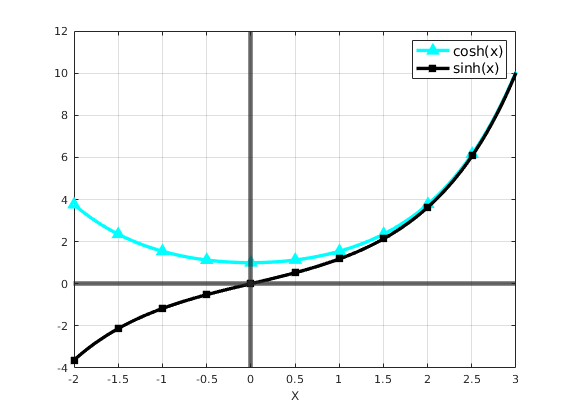
\includegraphics{cosh_and_sinh_plot.png}
\caption{Plot of $\cosh{x}$ and $\sinh{x}$}
\label{fig:cosh-and-sinh-plot}
\end{marginfigure}


For reasons that will become clear later in the course, it is sometimes useful to re-express the solution shown in Equation \ref{eq:sp-case-1-exp} in terms of the functions $\cosh$ and $\sinh$.  These functions are defined as linear combinations of exponentials as shown below and plotted in Figure \ref{fig:cosh-and-sinh-plot}
\begin{align*}
\cosh{x} &= \frac{e^{x} + e^{-x}}{2} \\
\sinh{x} &= \frac{e^{x} - e^{-x}}{2}
\end{align*}



\item \textbf{Real Repeated Roots}
In this case $m_1 = m_2$.\marginnote{i.e. from the quadratic equation, $b^2-4ac = 0$}  One solution is:
\begin{equation}
u_1(x) = e^{m_1x}
\end{equation}

The other solution so derived is, of course, the same and thus we do not have two linearly independent solutions as required to form a fundamental set of solutions for a 2\textsuperscript{nd}-order linear homogeneous equation.  

\newthought{It can be shown} that a second linearly independent solution can be formed by multiplying by the independent variable:\marginnote{This is done using a technique referred to as \emph{reduction of order}.  We will not take the time to cover it in this class (or in this book) but is concisely described in section 3.2 of Zill.  At a minimum you might at least confirm for yourself that a) $xu_1(x)$ is a solution to the equation; and b) use the Wronskian to confirm that it is linearly independent from $u_1(x)$.}
\begin{equation*}
u_2(x) = x u_1(x) = xe^{mx}
\end{equation*}
and thus the general solution for this case is:
\begin{equation}
u(x) = c_1e^{mx}+c_2xe^{mx}
\label{eq:rep-real-roots}
\end{equation}

\item \textbf{Conjugate Complex Roots}
In this case the discriminant, $b^2-4ac$, is negative so its square root is imaginary.  This results in $m_1$ and $m_2$ being complex conjugates which we will express as: $m_1 = \alpha + i\beta$ and $m_2 = \alpha - i\beta$.

The general solution is:
\begin{align*}
u(x) &= c_1e^{(\alpha + i\beta)x}+c_2e^{(\alpha - i\beta)x} \\
&=e^{\alpha x}\left(c_1e^{i\beta x} + c_2e^{-i\beta x} \right) 
\end{align*}

The complex exponentials in the last equation can be re-expressed using the Euler Formula:\index{Formula, Euler}
\begin{align*}
e^{i\beta x} &= \cos{\beta x} + i \sin{\beta x} \\
e^{-i\beta x} &= \cos{\beta x} - i \sin{\beta x}
\end{align*}
which is slighly more convenient insofar as the solutions are no longer expressed as complex exponentials but also by breaking each solution down into their real and complex parts. It can be shown that both the real and imaginary parts of the solution must satisfy the differential equation \emph{independently}.  This fact allows us to re-express the solution in a more simple form that does not involve complex numbers:
\begin{equation}
u(x) = e^{\alpha x}\left(c_1 \cos{\beta x} + c_2 \sin{\beta x} \right)
\label{eq:cmplx-conj-roots}
\end{equation}

\newthought{Another important} special case is when the solution is \emph{pure imaginary} (i.e. $\alpha = 0$) so the solution is:
\begin{equation}
u(x) = c_1 \cos{\beta x} + c_2 \sin{\beta x}
\end{equation}
These solutions arise when the governing equation is of the shown in Equation \ref{eq:special-case-2}:
\begin{equation}
u^{\prime \prime} + k^2 u = 0
\label{eq:special-case-2}
\end{equation}
The roots $m_{1,2} = \pm ik$ and the general solution is:
\begin{equation}
u(x)=c_1 \cos{kx} + c_2 \sin{kx}
\end{equation}
This equation will be revisited throughout the course as it repeatedly comes up in applications.
\end{enumerate}

\section{Three Examples}
The cases described above will be illustrated with three examples:

\vspace{0.5cm}
\noindent\textbf{Example \#1:}
Find the general solution to $2u^{\prime \prime}-5u^{\prime}-3u = 0$. Inserting $u = e^{mx}$ into the equation gives us the auxiliary equation:
\begin{equation*}
2m^2 - 5m - 3 = (2m+1)(m-3)
\end{equation*}
with roots: $m_1 = -\frac{1}{2}$ and $m_2 = 3$.  These are real, distinct roots so the general solution is:
\begin{equation*}
u(x) = c_1e^{-x/2}+c_2e^{3x}
\end{equation*}

\vspace{0.5cm}

\noindent\textbf{Example \#2:}
Find the general solution to $u^{\prime \prime}-10u^{\prime}+25u = 0$.
The auxiliary equation is:
\begin{equation*}
m^2-10m+25 = (m-5)(m-5)
\end{equation*}
with (repeated) roots: $m_1 = 5$ and $m_2 = 5$.  These are real, repated roots so the general solution is:
\begin{equation*}
u(x) = c_1e^{5x} + c_2xe^{5x}
\end{equation*}

\vspace{0.5cm}

\noindent\textbf{Example \#3:}
Find the general solution to $4u^{\prime \prime}+4u^{\prime} + 17u = 0, \ \ u(0)=-1, \ u^{\prime}(0)=2$.

This is an initial value problem\marginnote{We can see that it must be an \emph{initial} value problem because the conditions are both given at the same location, $x_0=0$.} with continuous (and constant) coefficients.  We know from Theorem \ref{thm:IVP-exist-and-unique} that a unique solution exists.  We will first find the general solution, then apply the initial conditions to resolve the unknown coefficients to reveal the solution.

The auxiliary equation is:
\begin{align*}
4m^2+4m+17 &= 0 \\
\text{using the quadratic equation, gives us:} \\
\frac{-4 \pm \sqrt{16 - 4(4)(17)}}{2(4)} &= -\frac{1}{2} \pm \frac{\sqrt{-256}}{8}\\
&= -\frac{1}{2} \pm \frac{-16}{8} \\
&= -\frac{1}{2} \pm 2i
\end{align*}
This gives us complex conjugate roots and the general solution is:
\begin{equation*}
u(x) = e^{-x/2}\left(c_1 \cos{2x} + c_2 \sin{2x} \right)
\end{equation*}
Applying the initial condition $u(0)=-1$ gives us:
\begin{align*}
u(0) &= e^{0}\left(c_1 \cos{0} + c_2 \sin{0} \right) \\
&= 1(c_1(1)+c_2(0)) \\
&= c_1 = -1
\end{align*}
To apply the second initial condition we need to use the chain-rule and product rule to differentiate the general solution.  This gives us:
\begin{multline*}
u^{\prime}(x) = -\frac{1}{2}e^{-x/2}c_1\cos{2x}-2e^{-x/2}c_1\sin{2x} + \\
-\frac{1}{2}e^{-x/2}c_2\sin{2x}+2e^{-x/2}c_2\cos{2x}
\end{multline*}
Evaluating $u^{\prime}(0)$ and substituting $c_1 = -1$ gives us:
\begin{align*}
u^{\prime}(0) &= -\frac{1}{2}(1)(-1)(1) + (1)(2)c_2(1) \\
&= \frac{1}{2}+2c_2 = 2 \\
  \Rightarrow 2c_2 &= \frac{3}{2} \\
 c_2 &= \frac{3}{4}
\end{align*}
Both constants are now known and the unique solution is:
\begin{equation*}
u(x) = e^{-x/2}\left(-\cos{2x}+\frac{3}{4}\sin{2x} \right)
\end{equation*}

\chapter{Lecture 5 - Non-homogeneous Linear Equations with Constant Coefficients}
\label{ch:lec5}
\section{Objectives}
The objectives of this lecture are:
\begin{itemize}
\item Describe the Method of Undetermined Coefficients for solving non-homogeneous linear equations with constant coefficients.
\item Carry out some examples to illustrate the methods.
\end{itemize}
In this lecture we will review \emph{a} method for finding solutions to non-homogeneous linear equations with constant coefficients.\marginnote{To be perfectly honest, we spend very little time in this class dealing with non-homogeneous equations of any kind; many of those types of equations are beyond our ability to solve analytically so we turn to numerical methods instead. Nonetheless there is value in reminding ourselves how to construct solutions for those cases where we can.}
\section{Background}
\newthought{Consider the equation} 
\begin{equation}
a_nu^{(n)} + a_{n-1}u^{(n-1)}+\cdots+a_1u^{\prime}+a_0u = g(x)
\label{eq:cc_nonhomo}
\end{equation}
where
\begin{itemize}
\item the coefficients $a_i, \ i\in [1,2,\dots,n]$ are constants; and
\item the function $g(x)$ is a constant, a polynomial function, exponential function, sine or cosine, or finite sums or products of these functions.
\end{itemize}
The general solution, $u(x)$, can be constructed as $u_c(x)+u_p(x)$ where
\begin{itemize}
\item $u_c(x)$ is the complementary solution which, as you should recall, is the general solution to the associated homogeneous problem. [i.e. Equation \ref{eq:cc_nonhomo} with $g(x)=0$]; and
\item $u_p(x)$ is (any) particular solution---that is, a not-necessarily-unique function that satisfies Equation \ref{eq:cc_nonhomo}.
\end{itemize}
We spent the last lecture describing, effectively, how to find $u_c(x)$; the question this lecture will hope to answer is: ``How do I find $u_p(x)$?''  
\section{Method of Undetermined Coefficients}\index{Undetermined Coefficients}
One method for finding $u_p(x)$ is called the Method of Undetermined Coefficients.\sidenote{Some people lovingly refer to this technique as "The Method of Guessing."}

\newthought{There are three} parts to this technique

\begin{enumerate}
\item \textbf{Basic Rule:} based on the terms in $g(x)$, select the appropriate form for $u_p(x)$ using Table \ref{tab:method-of-guessing-table}.

\begin{table}[h]
\begin{center}
\begin{tabular}{|c|l|}
%\toprule
\hline
Term in $g(x)$ & Choice for $u_p(x)$ \\\hline%\midrule

$ke^{\gamma x}$ & $Ae^{\gamma x}$ \\\hline
$kx^{n}, \ (n=0,1,\dots)$ & $K_nx^n+K_{n-1}x^{n-1}+\cdots +K_1x+K_0$\\\hline
$k \cos{\omega x}$ & \multirow{2}{*}{$\Big\} \ K\cos{\omega x} + M\sin{\omega x}$}\\\cline{1-1}
$k \sin{\omega x}$ &                 \\\hline
$ke^{\alpha x}\cos{\omega x}$   & \multirow{2}{*}{$\Big\} \ e^{\alpha x}\left(K\cos{\omega x} + M\sin{\omega x}\right)$}\\\cline{1-1} 
$ke^{\alpha x}\sin{\omega x}$ &      \\\hline
%\bottomrule
\end{tabular}
\end{center}
\caption{Forms of $u_p(x)$ for given terms in $g(x)$}
\label{tab:method-of-guessing-table}
\end{table}

\item \textbf{Modification rule:} if $u_p(x)$ obtained by the \textbf{Basic Rule} happens to be a solution to the associated homogeneous equation, multiply $u_p(x)$ from the table by $x$ (or $x^2$ if needed).

\item \textbf{Sum rule:} if $g(x)$ is a linear combination of terms from the left-hand column, construct $u_p(x)$ from a linear combination of the corresponding entries in the right-hand column.
\end{enumerate}
For the remainder of this lecture, we will practice applying these rules to some example problems.

\vspace{0.5cm}

\noindent{\textbf{Example:}} solve $u^{\prime \prime}+4u^{\prime}-2u = 2x^2 - 3x + 6$

\vspace{0.25cm}
\noindent{\textbf{Step \#1:}} find the general solution to the associated homogeneous equation.

\vspace{0.25cm}

\noindent The auxiliary equation is: $m^2 + 4m-2=0$; using the quadratic equation gives us:\marginnote{Here you are expected to examine the associated homogeneous problem as $u^{\prime \prime}+4u^{\prime}-2u =0$, identify it as constant coefficient and linear, and solve by assuming $u=e^{mx}$ and thus deriving the auxiliary equation shown without further prompting.} 
\begin{align*}
m &= \frac{-4 \pm \sqrt{16 - (4)(1)(-2)}}{2(1)} \\
&= -2 \pm \frac{\sqrt{24}}{2} \\
&= -2 \pm \sqrt{6}
\end{align*}
so $u_c(x) = c_1e^{(-2+\sqrt{6})x}+c_2e^{(-2-\sqrt{6})x}$

\vspace{0.25cm}
\noindent{\textbf{Step \#2:}} Apply the method of undetermined coefficients to construct a candidate $u_p(x)$.

\vspace{0.25cm}

\noindent Since $g(x)$ is a second-order polynomial, the table tells us $u_p(x)$ is in the general form of a second-order polynomial.
$$u_p(x) = K_2x^2+K_1x+K_0$$
We plug this into the governing equation and this gives us:
\begin{equation*}
2K_2 + 4(2K_2x+K_1) - 2(K_2x^2+K_1x+K_0) = 2x^2-3x+6
\end{equation*}
Now we need to equate the coefficient for each power of $x$:

\begin{table*}[h!]
\begin{tabular}{l r l}
$x^2$:&$-2K_2 $&$= 2$ \\
$x$:& $8K_2 - 2K_1$ &$= -3$ \\
$1$:&$2K_2+4K_1-2K_0$ &$= 6$
\end{tabular}
\end{table*}
Luckily for us, this system of equations is structured such that it can easily be solved.  We see by inspection that $K_2 = 2/-2 = -1$; this can be plugged into the second equation to find $K_1 = -5/2$ and then we can solve the last equation to find that $K_0 = -9$.\marginnote[-4.0cm]{In general you cannot expect this to go so nicely.  What you \emph{can} hope for is that the, in this case, three equations you derive will have a unique solution.  We could re-write the system in the form of a matrix-vector equation:
\begin{equation*}
\begin{bmatrix}
0 & 0 & -2 \\
0 & -2 & 8 \\
-2 & 4 & 2
\end{bmatrix}
\begin{bmatrix}
K_0 \\
K_1 \\
K_2
\end{bmatrix}
= 
\begin{bmatrix}
2 \\
-3 \\
6
\end{bmatrix}
\end{equation*}
If the solution of such a matrix cannot be done by inspection and simple algebra as it was in this case, we could use tools like MATLAB to solve the linear system of equations.  This topic and much more is covered in the numerical methods portion of this text.}

Thus the particular solution is:
\begin{equation*}
u_p(x) = -x^2-\frac{5}{2}x -9
\end{equation*}

\vspace{0.25cm}
\noindent\textbf{Step \#3:} Construct the general solution: $u(x) = u_c(x)+u_p(x)$.

\vspace{0.25cm}

\noindent We now have both the complementary solution and a particular solution; we form the general solution to the equation by adding them together.
\begin{align*}
u(x) &= u_c(x)+u_p(x) \\
&= c_1e^{(-2+\sqrt{6})x}+c_2e^{(-2-\sqrt{6})x}-x^2-\frac{5}{2}x -9
\end{align*}\marginnote[-1.5cm]{Why, again, do we need the constants $c_1$ and $c_2$?

\vspace{0.5cm}

\noindent\textbf{Answer: }Because we have not yet applied initial/boundary conditions.  If those conditions are provided---two conditions for a 2\textsuperscript{nd}-order problem---then we can resolve the constants.
}

\vspace{0.5cm}

\noindent\textbf{Example:} solve $u^{\prime \prime}-5u^{\prime}+4u=8e^x$

\vspace{0.25cm}

\noindent\textbf{Step \#1:} find the general solution to the associated homogeneous problem.

\vspace{0.25cm}

\noindent The auxiliary equation is $m^2-m+4=0$ the left side of which can easily be factored to give $(m-4)(m-1)=0$; the roots of which are $m_1=4$, $m_2=1$.  The complementary solution is:
\begin{equation*}
u_c(x) = c_1e^{4x}+c_2e^{x}
\end{equation*} 

\noindent\textbf{Step \#2:} Apply the method of undetermined coefficients to construct $u_p(x)$.

\vspace{0.25cm}

\noindent Inspecting Table \ref{tab:method-of-guessing-table} we see that $u_p(x)$ should be of the form $Ae^{x}$.  If that function seems vaguely familiar it may be because $e^x$ is part of the complementary solution. 

\vspace{0.25cm}

\noindent\textbf{Pop Quiz:} if you plug $Ae^{x}$ into your governing equation, without doing any calculations, what value should you get?

\vspace{0.25cm}

\noindent\textbf{Answer:} you will get zero!  Why? Because $e^{x}$ is one of the two linearly independent solutions to the associated homogeneous problem. 

\vspace{0.25cm}

\noindent\textbf{What do I do now?}

\vspace{0.25cm}

\noindent\textbf{Answer: } invoke the Modification Rule---this is, after all, the reason why the rule exists---and multiply $u_p$ by $x$.  We now have $u_p(x) = Axe^x$.

\vspace{0.25cm}

\noindent We insert this proposed function for $u_p(x)$ into the equation and we get:
\begin{equation*}
2Ae^x+Axe^x - 5(Ae^x+Axe^x) + 4Axe^x = 8e^x
\end{equation*} 
Combine terms and solve for $A$:
\begin{align*}
2Ae^x-5Ae^x &= 8e^x \\
-3Ae^x &= 8e^x \\
A &= -\frac{8}{3}
\end{align*}
So the particular solution is:
\begin{equation*}
u_p(x) = -\frac{8}{3}xe^x
\end{equation*}

\vspace{0.25cm}
\noindent\textbf{Step \#3:} Construct the general solution: $u(x)=u_c(x)+u_p(x)$.
\marginnote{\textbf{Note:} If any of this seems at all sketchy to you, the good news is that you need not worry if your proposed $u_p(x)$ is any good; you can just plug it into the differential equation and find out!}
\begin{align*}
u(x) &= u_c(x)+u_p(x) \\
&=c_1e^{4x}+c_2e^x - \frac{8}{3}xe^{x}
\end{align*}

\newthought{This last example} illustrates the use of the Sum Rule; it also includes initial condition so the unique solution to the initial value problem can be found.

\vspace{0.25cm}

\noindent\textbf{Example:} solve the initial value problem: $u^{\prime \prime}+u=4x+10\sin{x}$ with initial conditions $u(\pi)=0, \ u^{\prime}(\pi)=2$.

\vspace{0.25cm}

\noindent\textbf{Step \#1:} Find the general solution to the associated homogeneous problem.

\vspace{0.25cm}

\noindent The auxiliary equation is: $m^2+1=0$, therefore $m=\pm i$ and $u_c(x)$ can be found as:
\begin{equation*}
u_c(x) = c_1\cos{x}+c_2\sin{x}
\end{equation*}

\vspace{0.25cm}

\noindent\textbf{Step \#2:} Apply the method of undetermined coefficients to construct $u_p(x)$.

\vspace{0.25cm}

\noindent For this problem, $g(x) = 4x+10\sin{x}$ has two terms, so we will construct $u_p(x)$ using one term at a time; $u_{p_1}(x)$ using $4x$ and $u_{p_2}(x)$ using $10\sin{x}$.\marginnote[-1.0cm]{It's the linearity property of $\mathcal{L} = \frac{d^2}{dx}+1$ that makes this possible. If $\mathcal{L}(u_{p_1})=4x$ and $\mathcal{L}(u_{p_2})=10\sin{x}$ then $\mathcal{L}(u_{p_1}+u_{p_2})=4x+10\sin{x}$.}  

\vspace{0.25cm}

\noindent\textbf{Step \#2.a:} Find $u_{p_1}(x)$.

\vspace{0.25cm}

\noindent From Table \ref{tab:method-of-guessing-table}, for $g(x)=4x$, we should select $u_{p_1} = K_1x+K_0$.  Inserting this into the differential equation gives us: $K_1x + K_0 = 4x$.  By inspection we can see that $K_0 = 0$ and $K_1 = 4$ so $u_{p_1}(x) = 4x$.  

\vspace{0.25cm}

\noindent\textbf{Step \#2.b: } Find $u_{p_2}(x)$.

\vspace{0.25cm}

\noindent From Table \ref{tab:method-of-guessing-table}, for $g(x)=10\sin{x}$, we should select $u_{p_2} =  K\cos{x}+M\sin{x}$. Now that we have done this a couple of times we should be on the alert for portions of the complementary solution cropping up in our guesses for $u_p(x)$ so we immediately see that we must multiply $u_{p_2}$ by $x$.  If we do this and insert $Kx\cos{x}+Mx\sin{x}$ into the differential equation we get:
\begin{multline*}
\left(-2K-Mx\right)\sin{x}+\left(2M-Kx\right)\cos{x} + \dots \\ Kx\cos{x}+Mx\sin{x} = 10\sin{x}
\end{multline*}

\vspace{0.25cm}

\noindent Matching coefficients for $\sin{x}$ and $\cos{x}$ on both sides of the above equation leads us to conclude that $M=0$ and $-2K = 10$.  Therefore $K = -5$ and $u_{p_2}(x)=-5x\cos{x}$.\marginnote{Again, there is no harm in testing your proposed $u_{p_2}(x)$ to see if it does indeed produce the expected result.}

\vspace{0.25cm}

\noindent\textbf{Step \#3:} Construct the general solution: $u(x)=u_c(x)+u_p(x)$.

\begin{align*}
u(x) &= u_c(x) + u_p(x) \\ 
&= u_c(x) + u_{p_1}(x)+u_{p_2}(x) \\
&= c_1\cos{x}+c_2\sin{x}+4x-5x\cos{x}
\end{align*}

\newthought{All that remains} is to apply the initial conditions.  

\begin{align*}
u(\pi) &= c_1(-1)+c_2(0)+4\pi -5(\pi)(-1) \\
&=-c_1+9\pi = 0 \\
\Rightarrow &= c_1 = 9\pi
\end{align*}

\vspace{0.25cm}

\noindent Applying the initial condition $u^{\prime}=2$:
\begin{equation*}
u^{\prime}(\pi)=-9\pi(0)+c_2(-1)+4-5(-1)+5\pi(0)=2
\end{equation*}

\vspace{0.25cm}

\noindent Solving for $c_2$ gives us: $c_2 = 7$; folding this into the general solution:

\begin{equation*}
u(x) = 9\pi \cos{x}+7\sin{x}+4x-5x\cos{x}
\end{equation*}

\chapter{Assignment \#2}
\label{ch:ass2}
\begin{fullwidth}
The given family of functions is the general solution of the differential equation on the indicated interval.  Find a member of the family (i.e. find the values for the constants $c_1$ and $c_2$) that is a solution of the initial-value problem.

\begin{enumerate}[series=outerlist]
\item $u=c_1e^{x}+c_2e^{-x}; \ \ u^{\prime \prime}-u=0, \ u(0)=0, \ u^{\prime}(0)=1$

\vspace{1.0cm}

\item $u=c_1x + c_2x \ln{x}, \ \ (0,\infty), \ x^2u^{\prime \prime}-xu^{\prime}=0, \ u(1)=3, \ u^{\prime}(1)=-1$

\vspace{1.0cm}
\end{enumerate}

\noindent The given two-parameter family is a solution of the indicated differential equation on the interval $(-\infty,\infty)$.  Determine if a member of the family can be found that satisfies the boundary conditions.

\begin{enumerate}[resume=outerlist]
\item $u=c_1e^{x}\cos{x} + c_2e^{x}\sin{x}; \ \ u^{\prime \prime}-2u^{\prime}+3u=0$

\begin{enumerate}[series=innerlist]
\item $u(0)=1, \ u^{\prime}(\pi)=0$

\item $u(0)=1, \ u(\pi)=-1$

\item $u(0)=1, \ u(\pi/2)=1$

\item $u(0)=0, \ u(\pi)=0$
\end{enumerate}

\vspace{1.0cm}
\end{enumerate}
Determine if the given set of functions is linearly dependent or linearly independent on the interval $(-\infty,\infty)$.


\begin{enumerate}[resume=outerlist]
\item $f_1(x)=x, \ \ f_2(x)=x^2, \ \ f_3(x)=4x-3x^2$

\vspace{1.0cm}

\item $f_1(x)=1+x, \ \ f_2(x)=x, \ \ f_3(x)=x^2$
\vspace{1.0cm}
\end{enumerate}


\noindent Verify that the given two-parameter family of functions is the general solution of the non-homogeneous differential equation on the indicated interval.

\begin{enumerate}[resume]
\item $u^{\prime \prime}-7u^{\prime}+10u=24e^{x}, \ \ u=c_1e^{2x}+c_2e^{5x}+6e^{x}, \ \left(-\infty,\infty\right)$

\vspace{1.0cm} 

\end{enumerate}

\noindent Find the general solution to the given second-order differential equation.

\begin{enumerate}[resume]
\item $4u^{\prime \prime}+u^{\prime} = 0$

\vspace{1.0cm}

\item $u^{\prime \prime}-u^{\prime}-6u=0$

\vspace{1.0cm}

\item $u^{\prime \prime}+8u^{\prime}+16u=0$

\vspace{1.0cm}

\item $u^{\prime \prime}+9u=0$

\vspace{1.0cm}
\end{enumerate}


\noindent Solve the given initial-value problem.

\begin{enumerate}[resume]
\item $u^{\prime \prime}+16u=0, \ \ u(0)=2, \ u^{\prime}(0)=-2$

\vspace{1.0cm}

\item $u^{\prime \prime}-4u^{\prime}-5u=0, \ \ u(1)=0, \ u{\prime}(1)=2$

\vspace{1.0cm}

\item $u^{\prime \prime}+u =0, \ \ u^{\prime}(0)=0, \ u^{\prime}(\pi/2)=0$

\vspace{1.0cm}

\end{enumerate}

\noindent Solve the given differential equation using the Method of Undetermined Coefficients.

\begin{enumerate}[resume]
\item $u^{\prime \prime}-10u^{\prime}+25u=30x+3$

\vspace{1.0cm}

\item $u^{\prime \prime}+3u=-48x^2e^{3x}$

\vspace{1.0cm}
\end{enumerate}

\noindent Solve the given initial-value problem.

\begin{enumerate}[resume]
\item $5u^{\prime \prime} + u^{\prime} - 6x, \ \ u(0)=0, \ u^{\prime}(0)=-10$

\vspace{1.0cm}

\end{enumerate}

\noindent Solve the given boundary-value problem.

\begin{enumerate}[resume]
\item $u^{\prime \prime}+u=x^2+1, \ \ u(0)=5, \ u(1)=0$

\vspace{1.0cm}

\end{enumerate}

\noindent Solve the given initial-value problem in which the input function $g(x)$ is discontinuous. (\textbf{Hint:} Solve the problem on two intervals and then find a solution so that $u$ and $u^{\prime}$ are continuous at the boundary of the interval.)

\begin{enumerate}[resume]
\item $u^{\prime \prime}+4u=g(x), \ \ u(0)=1, \ u^{\prime}(0)=2$
\begin{equation*}
g(x) = 
\begin{cases}
\sin{x} & 0 \le x \le \pi/2 \\
0 & x > \pi/2
\end{cases}
\hspace{12cm}
\end{equation*}

\end{enumerate}


\end{fullwidth}



\part{Power Series Methods}


%%
% The back matter contains appendices, bibliographies, indices, glossaries, etc.

\part{Back Matter}
\backmatter

\bibliography{Mathematical_Methods_for_Engineers}
\bibliographystyle{plainnat}


\appendix
\appendixpage
\noappendicestocpagenum
\addappheadtotoc



\chapter{Matlab Style Rules}
\begin{enumerate}
\item \textbf{rule:} All scripts will start with the commands: \textbf{clear}, \textbf{clc}, and \textbf{close 'all'}

\textbf{rationale:} No script should depend upon any data visible in the MATLAB workspace when the script starts.  By omitting these commands, residual data within the workspace may hide errors.

\item \textbf{rule:} Your code must be documented with enough details such that a reader unfamiliar with your work will know what you are doing.

\textbf{rationale:} Code documentation is a habit. For more significant projects readers may need help in deciding what the author of the code intended.  For your own code, the most likely reader is you---a few months into the future.

\item \textbf{rule:} Function and variable names must be meaningful and reasonable in length.

\textbf{rationale:} Failing to do either make code harder to read and maintain.

\item \textbf{rule:} All outputs from the code \underline{\textbf{must}} be meaningful; numbers should be formatted, part of a sentence, and include units. Graphs should be readable and axis labels should make sense and include units.

\textbf{rationale:} Code output is a form of communication. It is important that this communication be clear and unambiguous.

\item \textbf{rule:} Do not leave warnings from the Code Analyzer unaddressed.

\textbf{rationale:} Sometimes Code Analyzer warnings can be safely ignored.  Most of the time the warning points to a stylistic error that would be unacceptable in software that you use. Occasionally these warnings are indicative of a hidden error.

\item \textbf{rule:} Use the ``smart indentation tool'' to format the indentation of your code.

\textbf{rationale:} This tool improves code readability. It will also occasionally point out errors that you did not see before.

\item \textbf{rule:} Pre-allocate arrays; if possible initialize with \textbf{NaN} values.

\textbf{rationale:} Pre-allocation improves performance and helps readability. Initialization with \textbf{NaN} helps avoid a range of potential logical errors.

\item \textbf{rule:} Avoid ``magic numbers'' --- i.e. hard-coded constants.

\textbf{rationale:} Constants included in your code tend to hide your program logic. Also, ``magic numbers'' make code maintenance more difficult and error prone.

\item \textbf{rule:} Only write one statement per line.

\textbf{rationale:} Multi-statement-lines hurt code readability in almost all cases.

\item \textbf{rule:} Do not write excessively long lines of code; use the line continuation ``...'' and indentation to spread long expressions over several lines.

\textbf{rationale:} Following this rule improves code readability.
\end{enumerate}


\printindex
\end{document}

